% This is the Duke University Statistical Science LaTeX thesis template.
% It has been adapted from the Reed College LaTeX thesis template. The
% adaptation was done by Mine Cetinkaya-Rundel (MCR). Some of the comments
% that are specific to Reed College have been removed.
%
% Most of the work on the original Reed College document class and template
% was done by Sam Noble (SN). Later comments etc. by Ben Salzberg (BTS).
% Additional restructuring and APA support by Jess Youngberg (JY).
%
% See https://www.reed.edu/cis/help/latex/ for help. There are a
% great bunch of help pages there, with notes on
% getting started, bibtex, etc. Go there and read it if you're not
% already familiar with LaTeX.
%
% Any line that starts with a percent symbol is a comment.
% They won't show up in the document, and are useful for notes
% to yourself and explaining commands.
% Commenting also removes a line from the document;
% very handy for troubleshooting problems. -BTS

%%
%% Preamble
%%
% \documentclass{<something>} must begin each LaTeX document
\documentclass[12pt,twoside]{dukestatscithesis}
% Packages are extensions to the basic LaTeX functions. Whatever you
% want to typeset, there is probably a package out there for it.
% Chemistry (chemtex), screenplays, you name it.
% Check out CTAN to see: http://www.ctan.org/
%%
\usepackage{graphicx,latexsym}
\usepackage{amsmath}
\usepackage{amssymb,amsthm}
\usepackage{longtable,booktabs,setspace}
\usepackage{chemarr} %% Useful for one reaction arrow, useless if you're not a chem major
\usepackage[hyphens]{url}
% Added by CII
\usepackage{hyperref}
\usepackage{lmodern}
\usepackage{float}
\floatplacement{figure}{H}
% End of CII addition
\usepackage{rotating}

% Next line commented out by CII
%%% \usepackage{natbib}
% Comment out the natbib line above and uncomment the following two lines to use the new
% biblatex-chicago style, for Chicago A. Also make some changes at the end where the
% bibliography is included.
%\usepackage{biblatex-chicago}
%\bibliography{thesis}


% Added by CII (Thanks, Hadley!)
% Use ref for internal links
\renewcommand{\hyperref}[2][???]{\autoref{#1}}
\def\chapterautorefname{Chapter}
\def\sectionautorefname{Section}
\def\subsectionautorefname{Subsection}
% End of CII addition

% Added by CII
\usepackage{caption}
\captionsetup{width=5in}
% End of CII addition

% \usepackage{times} % other fonts are available like times, bookman, charter, palatino


% To pass between YAML and LaTeX the dollar signs are added by CII
\title{Examining Injustice in Environmental Toxicity}
\author{Anne Driscoll}
% The month and year that you submit your FINAL draft TO THE LIBRARY (May or December)
\date{May 2018}
\advisor{David Banks}
\institution{Duke University}
\degree{Bachelor of Science in Statistical Science}
\committeememberone{Committeemember O. Name}
\committeemembertwo{Committeemember T. Name}
\dus{Mine Cetinkaya Rundel}
%If you have two advisors for some reason, you can use the following
% Uncommented out by CII
% End of CII addition

%%% Remember to use the correct department!
\department{Department of Statistical Science}

% Added by CII
%%% Copied from knitr
%% maxwidth is the original width if it's less than linewidth
%% otherwise use linewidth (to make sure the graphics do not exceed the margin)
\makeatletter
\def\maxwidth{ %
  \ifdim\Gin@nat@width>\linewidth
    \linewidth
  \else
    \Gin@nat@width
  \fi
}
\makeatother

\renewcommand{\contentsname}{Table of Contents}
% End of CII addition

\setlength{\parskip}{0pt}

% Added by CII
  %\setlength{\parskip}{\baselineskip}
  \usepackage[parfill]{parskip}

\providecommand{\tightlist}{%
  \setlength{\itemsep}{0pt}\setlength{\parskip}{0pt}}

\Acknowledgements{
I want to thank a few people.
}

\Dedication{
You can have a dedication here if you wish.
}

\Preface{
This is an example of a thesis setup to use the reed thesis document
class (for LaTeX) and the R bookdown package, in general.
}

\Abstract{
The preface pretty much says it all. \par

Second paragraph of abstract starts here.
}

% End of CII addition
%%
%% End Preamble
%%
%

\usepackage{amsthm}
\newtheorem{theorem}{Theorem}[chapter]
\newtheorem{lemma}{Lemma}[chapter]
\theoremstyle{definition}
\newtheorem{definition}{Definition}[chapter]
\newtheorem{corollary}{Corollary}[chapter]
\newtheorem{proposition}{Proposition}[chapter]
\theoremstyle{definition}
\newtheorem{example}{Example}[chapter]
\theoremstyle{definition}
\newtheorem{exercise}{Exercise}[chapter]
\theoremstyle{remark}
\newtheorem*{remark}{Remark}
\newtheorem*{solution}{Solution}
\begin{document}

% Everything below added by CII
  \maketitle

\frontmatter % this stuff will be roman-numbered
\pagestyle{empty} % this removes page numbers from the frontmatter
  \begin{acknowledgements}
    I want to thank a few people.
  \end{acknowledgements}
  \begin{preface}
    This is an example of a thesis setup to use the reed thesis document
    class (for LaTeX) and the R bookdown package, in general.
  \end{preface}
  \hypersetup{linkcolor=black}
  \setcounter{tocdepth}{2}
  \tableofcontents

  \listoftables

  \listoffigures
  \begin{abstract}
    The preface pretty much says it all. \par
    
    Second paragraph of abstract starts here.
  \end{abstract}
  \begin{dedication}
    You can have a dedication here if you wish.
  \end{dedication}
\mainmatter % here the regular arabic numbering starts
\pagestyle{fancyplain} % turns page numbering back on

\chapter*{Introduction}\label{introduction}
\addcontentsline{toc}{chapter}{Introduction}

Environmental justice literature has focused largely on the motivations
behind facility siting that lead to inequality and policy approaches to
help fix the disproportionate burden of environmental hazards on
minority communities. The questions being asked are critical to creating
policy that helps correct the problem of hazard allocation. A gap in the
literature is the need for an investigation of the dynamic world of
hazard allocation over time.

*what is natural sorting

*How are env dumps created?

*Breaking the self fulfilling cycle

\textless{}\textless{}\textless{}\textless{}\textless{}\textless{}\textless{}
HEAD This thesis seeks to address the question of how the toxicity
experienced by minority communities has changed. Specifically, we look
for substantial reductions in relative environmental toxicity, when
shifts are occur, and what traits that are predictive of high
environmental toxicity.

\subsection{Keywords}\label{keywords}

\chapter{Environmental Inequality, Racial Inequality, Non-parametric
analysis}\label{environmental-inequality-racial-inequality-non-parametric-analysis}

This thesis seeks to address the investigative question of if minority
communities have experienced substantial reductions in their relative
environmental toxicity, when those shifts are occuring, and a look in to
the traits that are predictive of high environmental toxicity.
\textgreater{}\textgreater{}\textgreater{}\textgreater{}\textgreater{}\textgreater{}\textgreater{}
master

\chapter{Introduction to Environmental Justice}\label{rmd-basics}

\chapter{Data}\label{math}

\section{Raw Data}\label{raw-data}

The Risk Screening Environmental Indicators (RSEI) Model is a
geographically detailed data set produced by the Environmental
Protection Agency (EPA). RSEI data is based upon the Toxic Release
Inventory (TRI), which (for about 30 years) has been collecting data on
all toxic releases in the US. The TRI program manages the regulations,
policies and facilities that ultimately are mandated to be reported.

TRI data is self reported by facilities, with each observation being a
release of a reporting chemical at a reporting facility. For each
observation, data is collected on which chemical was released, how much
of it was released, and the facility from which it was released.

The detailed location and chemical data that is collected through TRI
(as well as detailed weather data from NOAA) is reformatted through a
fate and transport model to create RSEI. The RSEI data shows where each
release has traveled on an 800m grid across the USA. The ultimate data
we have access to through the RSEI data is an observation for each
release, for each square in the grid that the release hits. This gives
us an idea of how the chemicals spread from the release locations, and
enables us to create a map across the entire nation for where TRI
chemicals accumulate in any year between 1988 and 2014.

The initial data from RSEI is in the form of one observation per release
per block on the 800m grid that it reached. Given that the 800m grid
across the United States has on the order of 10 billion squares, each
release hits many squares, we have many releases, and the data covers 27
years, this is an enormous data set. Overall, the disaggregated
microdata is approximately 4 terabytes of data.

The RSEI reformat of the TRI provides some additional information
computed from the release information, and additional geographic
information. X and Y are the geographic identifiers for the square on
the grid across the US, with (0, 0) in the center of the US. Release
number tells us which release that row is associated with. Chemical
number through media are all release specific data, but all data beyond
that is release and grid number specific. Conc (concentration) is the
raw concentration of the amount of the chemical that reached that grid
cell. ToxConc is the toxicity weighted concentration of that release in
that grid cell. The various `Score' variables are meant to be used as
hazard created by that release in that grid cell, as they are weighted
by the population in that grid cell.

Below see an example of the disaggregated microdata:
\begin{longtable}[]{@{}llllllllllll@{}}
\toprule
X & Y & Release & Chem & Facility & Media & Conc & ToxConc & Score &
SCancer & SNoCan & Pop\tabularnewline
\midrule
\endhead
-185 & 51 & 2050156 & 317 & 3 & 1 & 4.55e-4 & 2.28e-3 & 0 & 0 & 0 &
0\tabularnewline
-184 & 41 & 2050156 & 317 & 3 & 1 & 3.29e-4 & 1.65e-3 & 0 & 0 & 0 &
0\tabularnewline
-184 & 42 & 2050156 & 317 & 3 & 1 & 3.33e-4 & 1.67e-3 & 0 & 0 & 0 &
0\tabularnewline
-184 & 43 & 2050156 & 317 & 3 & 1 & 3.33e-4 & 1.66e-3 & 0 & 0 & 0 &
0\tabularnewline
-184 & 44 & 2050156 & 317 & 3 & 1 & 3.35e-4 & 1.68e-3 & 0 & 0 & 0 &
0\tabularnewline
\ldots{} & \ldots{} & \ldots{} & \ldots{} & \ldots{} & \ldots{} &
\ldots{} & \ldots{} & \ldots{} & \ldots{} & \ldots{} &
\ldots{}\tabularnewline
\bottomrule
\end{longtable}
\section{Important Caveats}\label{important-caveats}

Due to the nature of the data, there are a few interesting caveats to
consider.
\begin{itemize}
\item
  The RSEI data is self reported, and has been thought to contain some
  severe underreporting.
\item
  The data is entirely based off a black box fate and transport model.
  The model has uncertainty that we are not addressing.
\item
  The data only captures releases for certain facility types within
  certain industries, for certain chemical types within those
  facilities. Not all chemicals are mandated reporting, and any analysis
  that is done based off the data can't be extrapolated to discuss
  toxicity more generally.
\item
  Not only does the data not capture all chemicals, it also doesn't
  adress many common nuicances. Because of this, it is difficult to
  relate the RSEI scores to health or quality of life outcomes in an
  area. In discussion of environmental toxicity more generally, it is
  worth noting that certain toxicity types may be more or less likely to
  cause adcerse effects based on how they reach people in the area (eg.
  they may or may not reach local water systems). There are also more
  obvious environmental hazards, that are likely to have strong
  influence on public health and living conditions that TRI doesn't
  address, eg: brownfields, solid waste disposal, animal farming,
  hazardous waste, etc.
\item
  RSEI gives the weight of the release and the chemical of the release,
  but chemicals have very different levels of toxicity. A small amount
  of mercury released is much more problematic than a small amount of
  CO2. To that end, the EPA assigned each chemical a `toxicity' weight,
  by which the amount of the chemical released is multiplied. This means
  that we can aggregate all the chemicals in an area, and compare the
  overall toxicity over space and time. The toxicity weights allow us to
  compare to other chemicals' toxicity weight, and overall toxicity of a
  given chemical release, but also means that the values only have
  meaning in comparison.
\end{itemize}
Despite the limitations that the data presents, it provides an
incredibly detailed and complex view of toxicity in America that is
worth delving in to.

\section{Consistency in Reporting (detailed data
description)}\label{consistency-in-reporting-detailed-data-description}

\subsection{Census Comparability}\label{census-comparability}

For the time period that RSEI data is available for (1988 - 2014),
Census geographies have experienced considerable overhaul. Many of our
questions of interest involve demographic characteristics, and the
changes we see in environmental toxicity over time for those
demographics. As such, we need to be able to aggregate the toxicity to
block group or tract level to be able to merge with Census data. To do
so, we caluclate the toxicity values for each geographic unit for the
closest temporal census geography (1990, 2000 or 2010). If we want to
use Census areas as the unit of analysis, we also need to consider
consistency of the units definition over time. To do so we would need to
create crosswalks that help us transform past Census geographies to the
current form, allocating the population appropriately to the new
geographies.

\subsection{Details of Chemical
Consistency}\label{details-of-chemical-consistency}

Comparability across time, space, and chemicals is a consistent topic
through this section. The EPA is incredibly detailed in their data
collection, and creation of metrics to make the data meaningful on a
broad scale. Unfortunately the EPA is subject to the changing scientific
consensus of the times, and therefore hasn't been able to provide
entirely consistent data.

Over time, as chemicals have been found to be toxic, they have been
added to the list of TRI mandated reporting chemicals. There are also
chemicals that through renewed understanding have been removed from the
mandated reporting list. Because the list of chemicals reported changes
over time, aggregating all the data would cause us to see artificial
jumps in toxicity. These jumps wouldn't be reflective of an actual
increase in toxicity, but rather that the toxicity was beginning to be
measured. These jumps may change what areas appear as toxic i the data,
as industries that don't have to report at some point in the time frame
will be entirely removed from the dataset. Several of those industries
are very highly polluting, areas who focus strongly on those industries
will show inaccurate low scores.

\subsection{Details of Industry Reporting
Consistency}\label{details-of-industry-reporting-consistency}

TRI regulates who needs to self report using the North American Industry
Classification System (NAICS), and before NAICS was available used its
predecessor, the Standard Industrial Classification (SIC) system. Just
as we see changes in the regulations for chemicals, we see changes in
the regulations of various industries. NAICS codes that need to report
are regulated independently of chemical codes, and NAICS codes that are
not consistently reported across the time period of interest must be
removed to maintain continuity. For a toy example, a textiles facility
releasing mercury might have to report it, but the neighboring mining
facility might not have to report their mercury emissions. If that
changes over the time period, and suddenly mining needs to report, we
will see an artificial huge jump in the mercury present in that area if
we don't remove by industry.

\section{Ultimate Data Form}\label{ultimate-data-form}

The disaggregated microdata from RSEI is one observation per release per
block on the 800m grid that it reached. The munging for these 4
terabytes of data filters each of the billions of observations to check
that it is 1) from a chemical that is consistent across the relevant
years 2) from an released that is linked to an industry that is
consistent across years, and 3) allocates the observation to the
appropriate geography.

This data cleaning is done through R, using the DBI and SQLite packages.
Since there is so much data, it's not feasible to process it using
typical R function, so after loading the data in to a database, it
becomes queryable using SQL. This significantly speeds up the processes
detailed below.

To accomplish the chemical consistency, we use a data table (provided by
Rich Puchalsky) that contains a row for each chemical with the data of
regulation, and the date of deregulation. Using this information, we can
select the chemicals that are relevant to any set of years of interest.
Chemicals are found by selecting the subset of chemicals where the year
of initial regulation is before the interest period, and the year of
deregulation is after the interest period, while also excluding delisted
chemicals, and all observations are checked to be in this range.

Filtering out observations whose releases are not under a regulated
NAICS category for the entire time is more complex. Using a similar
table that contains the regulation and deregulation dates of NAICS codes
we can find the consistent industry categories. However, the only
reference to NAICS or SIC codes are in the facility table that the
releases reference. This table provides 6 NAICS codes that are the most
common NAICS codes associated with the facility. However, NAICS codes
are release specific, not facility specific, meaning that for each
emission reported a NAICS code is reported. Removing by facility is not
accurate, since facilities might have different types of NAICS
emissions. The textiles facility we used as an example earlier might
make both shoes and jackets, with different industry codes and different
releases that have different reporting requirements. To get data on the
NAICS codes by submission, data must be taken from the original TRI
data, and linked to the disaggregated microdata by the document control
number.

In the data cleansing process, we filter the data to remove industries
and chemicals that were not consistent over the period of inquiry, and
aggregate the data to the relevant Census geographies. The data, then
forms a data set for each year, with an observation for each block
group, and just one measure, an aggregated toxicity level.
\begin{longtable}[]{@{}lll@{}}
\toprule
block & concentration & area\tabularnewline
\midrule
\endhead
010010201001 & 627.3050138 & 6.520168\tabularnewline
010010201002 & 499.6297799 & 8.48669\tabularnewline
010010202001 & 578.8311689 & 3.137173\tabularnewline
010010202002 & 756.3733114 & 1.962949\tabularnewline
010010203001 & 637.7356488 & 5.907125\tabularnewline
\ldots{} & \ldots{} & \ldots{}\tabularnewline
\bottomrule
\end{longtable}
The `concentration' estimate must be interpreted in the context of the
consistency adjustments. For example, towns with extremely high mining
emissions may not show as exceptionally high pollution, as mining is one
of the industries that had different regulations over the 1990-2010 time
period, and therefore the reported mining emissions have been removed
entirely. Essentially, the pollution estimates are comparable across
time and location, but only in the context of continuous EPA regulation,
and can not be interpreted independently of one another.

\chapter{Approaches and Methods}\label{ref-labels}

\section{Geographic Level of
Analysis}\label{geographic-level-of-analysis}

The questions we would like to pose - how the distributions of toxicity
that individuals experience over time are predicted by their complex,
multidimensional identities - is inherently intended to be a person
level analysis. That intent may not be achievable given the available
data.

This analysis depends on two data sources, the disaggregated RSEI toxic
release data (as compiled to contain only releases that are consistently
reported between 1990 and 2010) as well as relevant demographic
information from the Census.

RSEI toxicity data can be obtained at extremely fine level (the 800
meter grid across the United States,) but the finest grain Census data
is available at is the block level, which contains between 0 and a few
hundred people. At such low geographic levels, few variables are
available for demographics due to identifiability concerns. At low
levels cross tabulations are not available due to concerns of
identifiability. Using a low level of geography (like census blocks or
block groups) is important for the environmental aspect of this
analysis, since environmental hazards can be very localized, especially
along neighborhood lines in urban areas.

Unfortunately, the availability of cross tabulations is equally
important to the goal of this work in examining inequality of
environmental burden held by minority groups in America. The
intersection of social identies, especially those steeped in systems of
oppression, is extremely important for identifying unequal burdens. For
example, low income populations across the board may be more likely to
experience environmental hazards, but low income minority populations
could be much more likely than low income white populations to
experience extreme hazard. The intersections of demographic
charictersitics, such as race and income or race and education are
likely to be important in teasing out differences true inequality
burden.

We combine the computed aggregated toxicity for each block group and the
demographic data. Now for each census geography, we have toxicity
information as well as demographic data.
\begin{longtable}[]{@{}llllll@{}}
\toprule
block & concentration & area & total\_pop & white & black\tabularnewline
\midrule
\endhead
010010201001 & 627.3050 & 6.520168 & 530 & 447 & 83\tabularnewline
010010201002 & 499.6298 & 8.486690 & 1282 & 1099 & 126\tabularnewline
010010202001 & 578.8312 & 3.137173 & 1274 & 363 & 824\tabularnewline
010010202002 & 756.3733 & 1.962949 & 944 & 458 & 477\tabularnewline
010010203001 & 637.7356 & 5.907125 & 2538 & 2152 & 384\tabularnewline
\ldots{} & \ldots{} & \ldots{} & \ldots{} & \ldots{} &
\ldots{}\tabularnewline
\bottomrule
\end{longtable}
To move to a person level analysis, we can assign each of the people the
toxicity for the geography they originated in. By assigning each person
the toxicity of their block group, we can aggregate nationally to find
the distribution of toxicity that each group experiences. This approach
is restricted in ability to approach the problem in an intersectional
manner, since we can only build a distribution for each of the crosstabs
we have available. For higher levels of geography (where we might, for
example, have race by income) we would be able to build national
distributions for each income by race group. In the case of the table
above, to build a distribution for the white population, we would assing
447 people a toxicity of \textasciitilde{}627, 1099 people a toxicity of
\textasciitilde{}499 and so on until we have the full distribution of
toxicities experienced by the white population. In choosing the level of
aggregation at which to assign toxicity, in order to balance the needs
of accuracy of toxicity and availability of cross tabulations, we create
the overall toxicity distribution for Americans at each of the levels of
geography. The process described above can be excecuted with the data
shown above, or at a cruder level of geography, such as state. Using
block group as the smallest form of geography, and state as the largest
(including tract and county in between) we see how the distribution
changes at each level of aggregation.

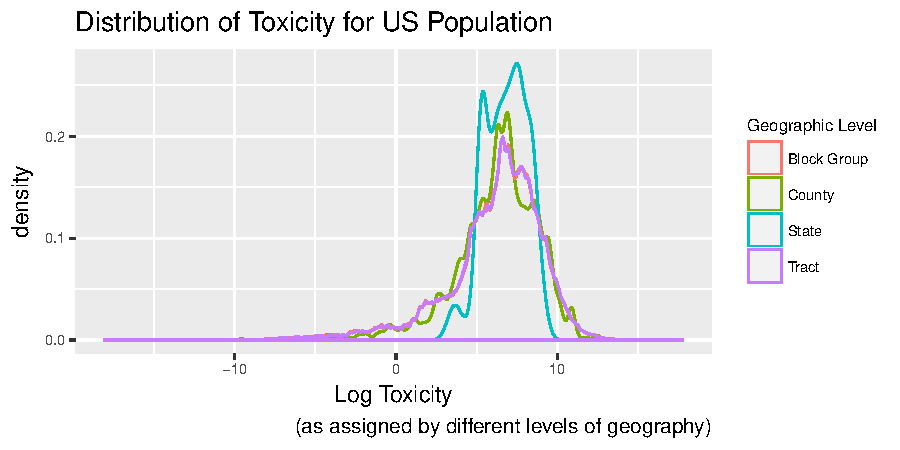
\includegraphics{thesis_files/figure-latex/unnamed-chunk-2-1.pdf}

As expected, the state level assignment is a poor approximation of the
lower level assignments. Given that we are assigning each individual the
mean toxicity in their entire state, we are eliminating most of the
variation from the data. Interestingly the tract data seems to build a
distribution very similar to the block group level assignment. This may
be because the block group level is aggregating a large enough group of
our fine grain toxicity data that it lost the street block by street
block variation that we had deemed so crucial, so aggregating several
block groups gives us a conceptual equivalent `neighborhood' level of
aggregation.

\section{Non-Parametric Analysis}\label{non-parametric-analysis}

To examine the change of environmental burden over time for groups we
first use a non-parametric simulation technique to tease apart the
forces in play as each group's distribution changes over time. For any
given value, the percentile it holds in a minority distribution is
likely to be different from the percentile it holds in the overall
distribution. For example, in 2010 the 75th percentile of the black
distribution is 2528.45, while that same value is the 81.44th percentile
in the overall distribution.

We expect the mean of minority distributions to reduce over time for two
reasons: first we assume the entire distribution will slowly be shifting
right as we see improvements in environmentally friendly production
technology and more comprehensive envirnmental regulation. Secondly, we
hope that with Title VI protetections, and the work of civil rights
advocates, minority communities will better protected against the
economic power frequently held by polluters.

In order to track how minority distribution and the overall distribution
have changed over the period of study, we use the positions that
minority groups held in the overall distribution at the start of the
period of study to simulate how each group's distribution would have
progressed through time assuming a static position in society at large.
This simulation proceeds as follows:
\begin{itemize}
\item
  Build an emipirical distribution of toxicity experienced for the
  entire population and for groups of interest in the starting year.
\item
  Sample individuals from the empirical distributions for the entire
  population and the groups of interest.
\item
  For each sampled value, find the percentile in the empirical
  distribution for the entire population in the starting year.
\item
  Create an empirical distribution for the entire population in the
  ending year.
\item
  For each sampled percentile, find the corresponding value in the full
  empirical distribution of the ending year and assign to the
  appropriate group of interest.
\end{itemize}
Using this method we can hold constant the place each individual (and
more broadly each group) holds in the overall distribution, but follow
the changes in the distribution as a whole. The collection of values
simulated now represents where each individual or group would have been
had there been no positional improvement for the group as a whole.

If there had been improvement for a group, we would expect the simulated
distributions to paint a bleaker picture of the environmental burden
borne than the true distribution of the ending year.

\section{Temporal Level of Analysis}\label{temporal-level-of-analysis}

Given the layout of this non-parametric method, we can find the changes
in positional distribution for any two given years. Though we are most
interested in the complete change from the starting year of 1988 to
2014, as that is the data we have, the gradual changes and the speed of
change from year to year is also of interest. While we have the full
range of data from 1988 to 2014 for the toxicity data, we only have
available Census data from the decennial census and the ACS. That means
that we have snapshots of data from 1990, 2000, and continuous data for
2010 on.

\section{Trends Over Time}\label{trends-over-time}
\begin{verbatim}
Parsed with column specification:
cols(
  year = col_integer(),
  white_sd = col_double(),
  black_sd = col_double(),
  asian_sd = col_double(),
  native_sd = col_double(),
  other_sd = col_double()
)
Parsed with column specification:
cols(
  year = col_integer(),
  white_sd = col_double(),
  black_sd = col_double(),
  asian_sd = col_double(),
  native_sd = col_double(),
  other_sd = col_double()
)
Parsed with column specification:
cols(
  year = col_integer(),
  white_sd = col_double(),
  black_sd = col_double(),
  asian_sd = col_double(),
  native_sd = col_double(),
  other_sd = col_double()
)
\end{verbatim}
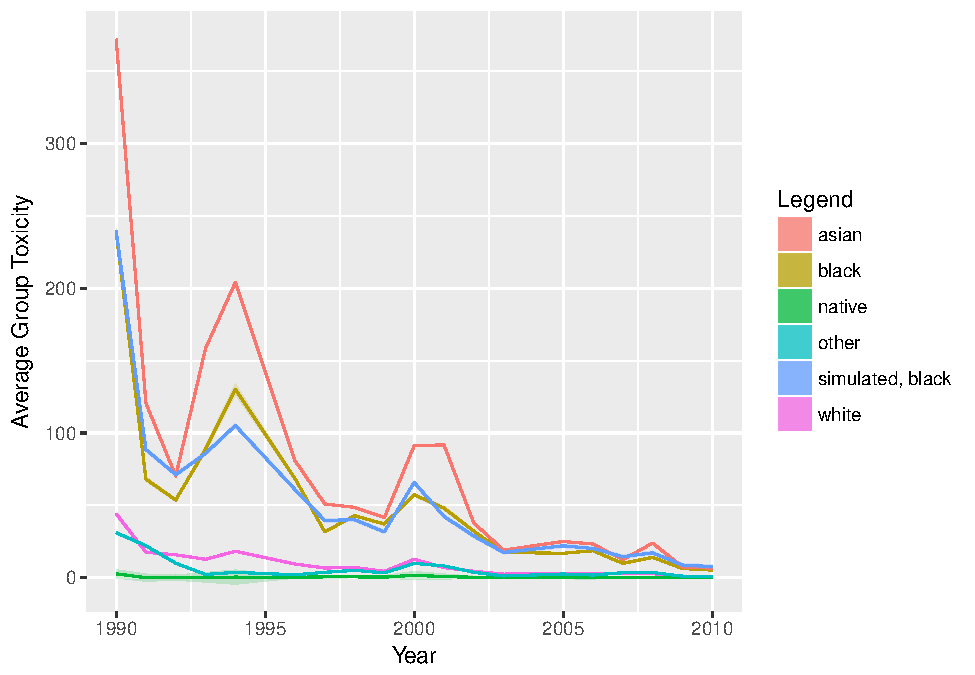
\includegraphics{thesis_files/figure-latex/unnamed-chunk-4-1.pdf}
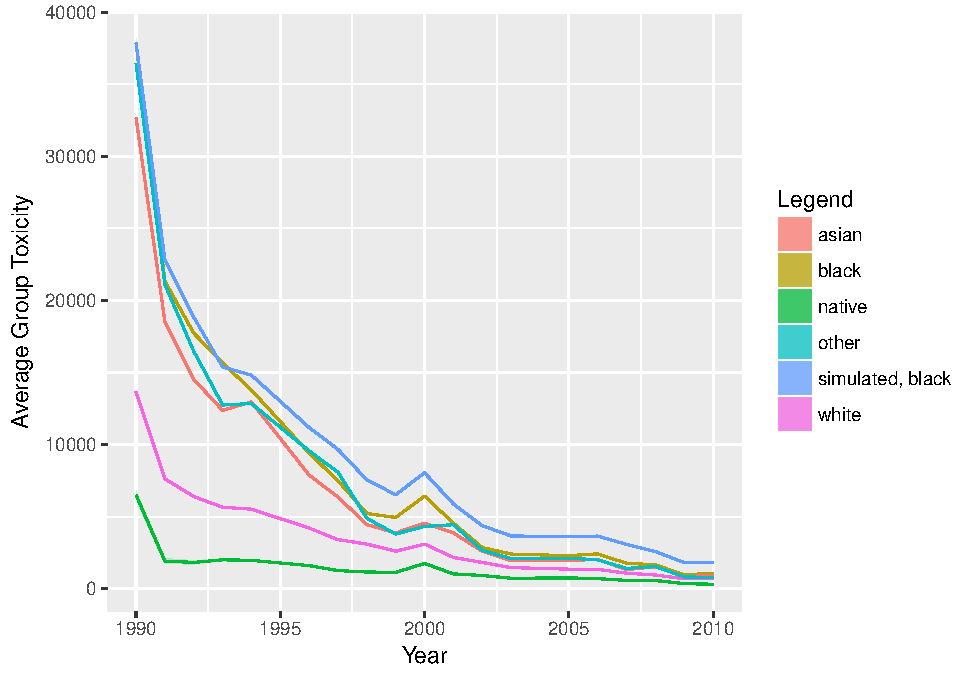
\includegraphics{thesis_files/figure-latex/unnamed-chunk-4-2.pdf}
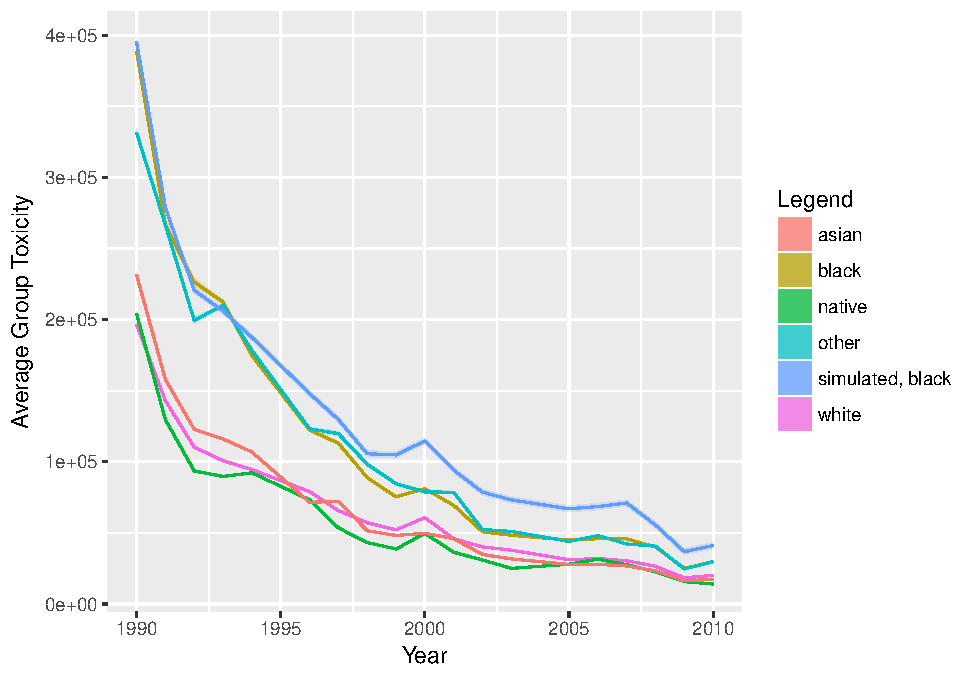
\includegraphics{thesis_files/figure-latex/unnamed-chunk-4-3.pdf}
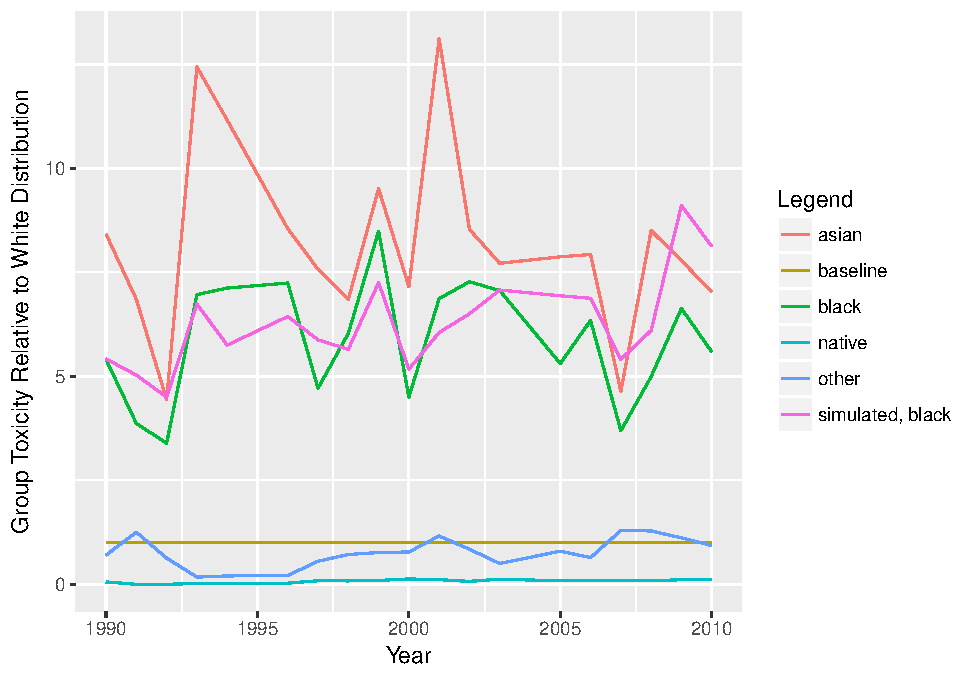
\includegraphics{thesis_files/figure-latex/unnamed-chunk-4-4.pdf}
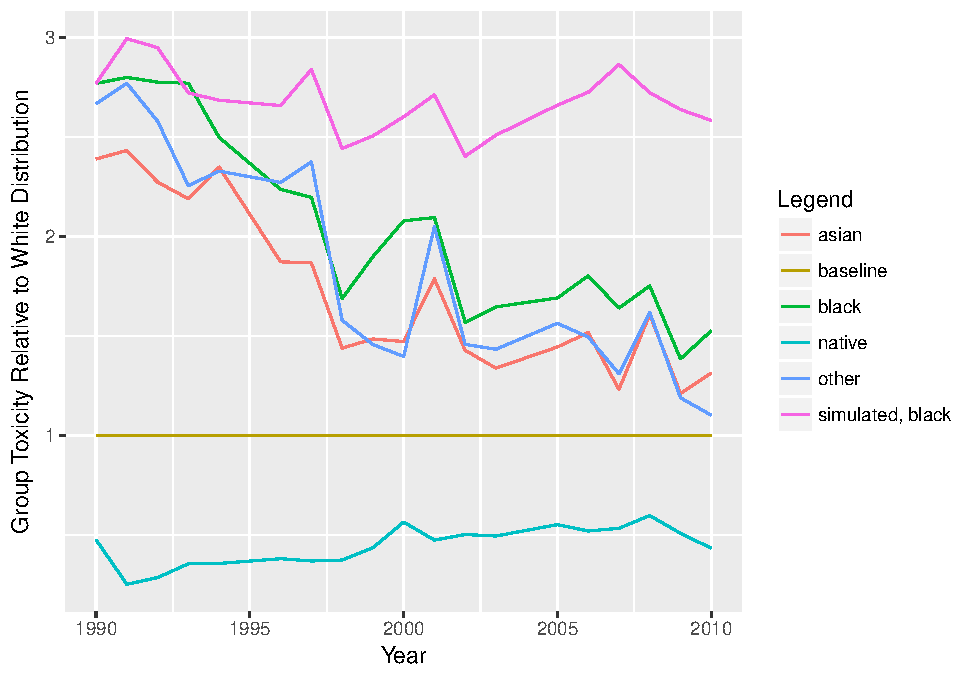
\includegraphics{thesis_files/figure-latex/unnamed-chunk-4-5.pdf}
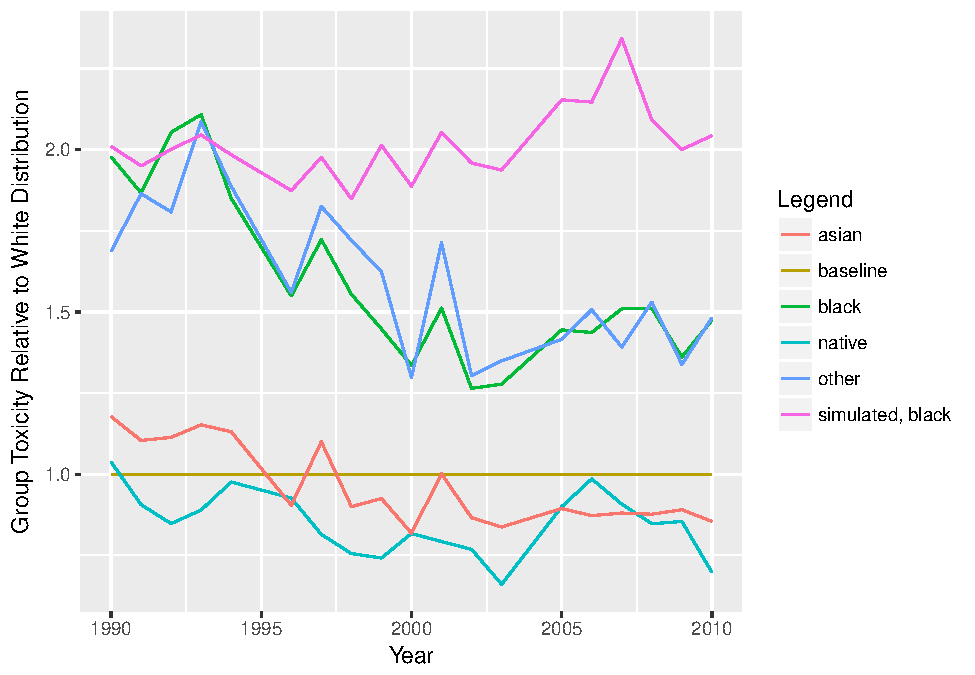
\includegraphics{thesis_files/figure-latex/unnamed-chunk-4-6.pdf}
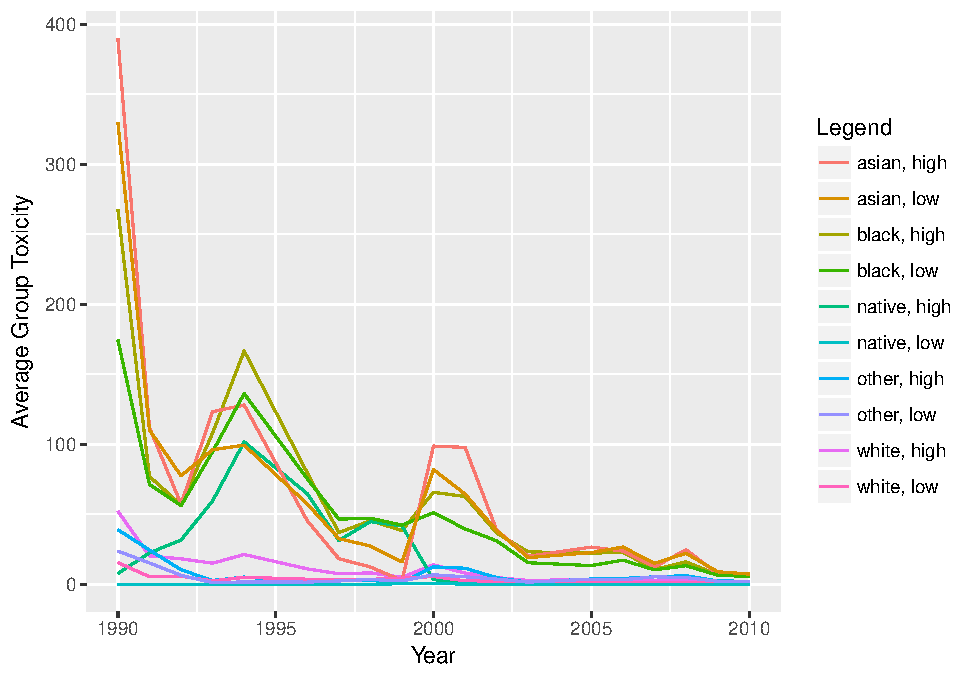
\includegraphics{thesis_files/figure-latex/unnamed-chunk-4-7.pdf}
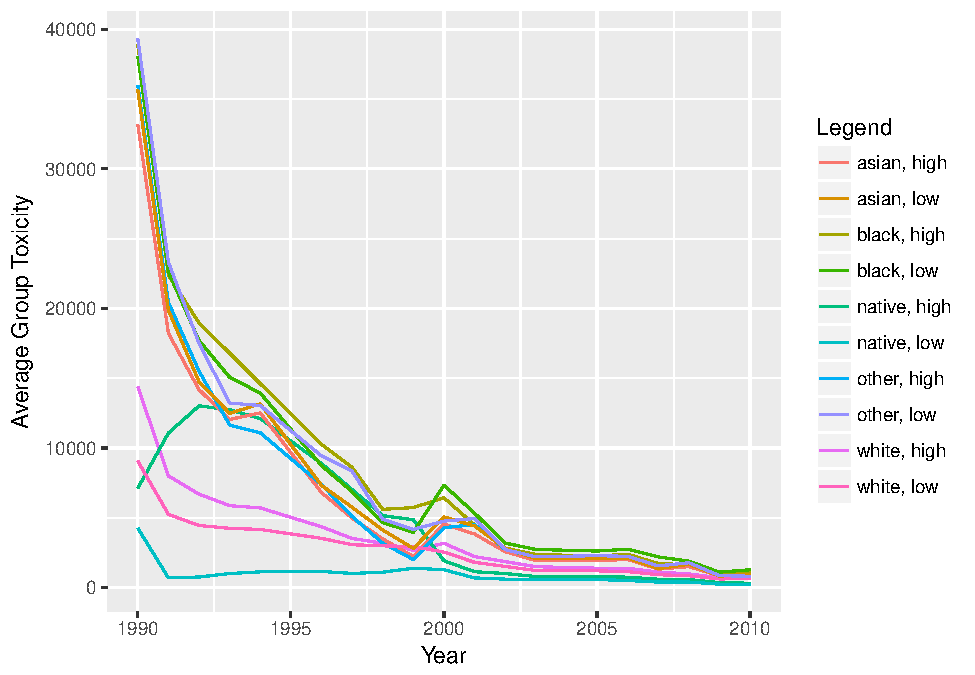
\includegraphics{thesis_files/figure-latex/unnamed-chunk-4-8.pdf}
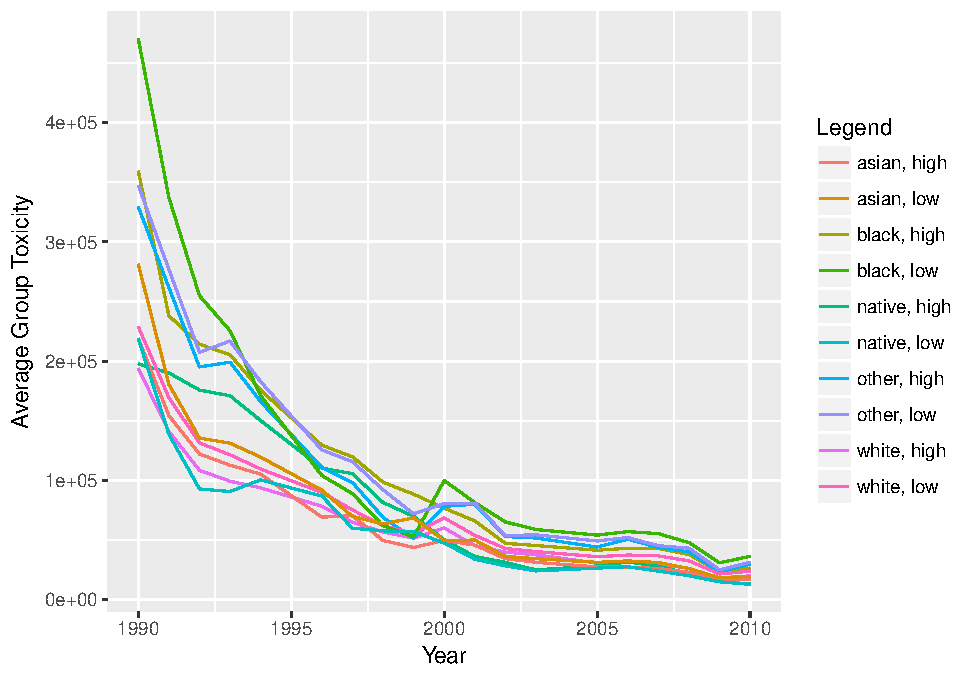
\includegraphics{thesis_files/figure-latex/unnamed-chunk-4-9.pdf}

\subsection{Notes on Simulation}\label{notes-on-simulation}
\begin{verbatim}
Parsed with column specification:
cols(
  n = col_integer(),
  sd = col_double(),
  mean = col_double()
)
Parsed with column specification:
cols(
  n = col_integer(),
  sd = col_double(),
  mean = col_double()
)
Parsed with column specification:
cols(
  n = col_integer(),
  sd = col_double(),
  mean = col_double()
)
\end{verbatim}
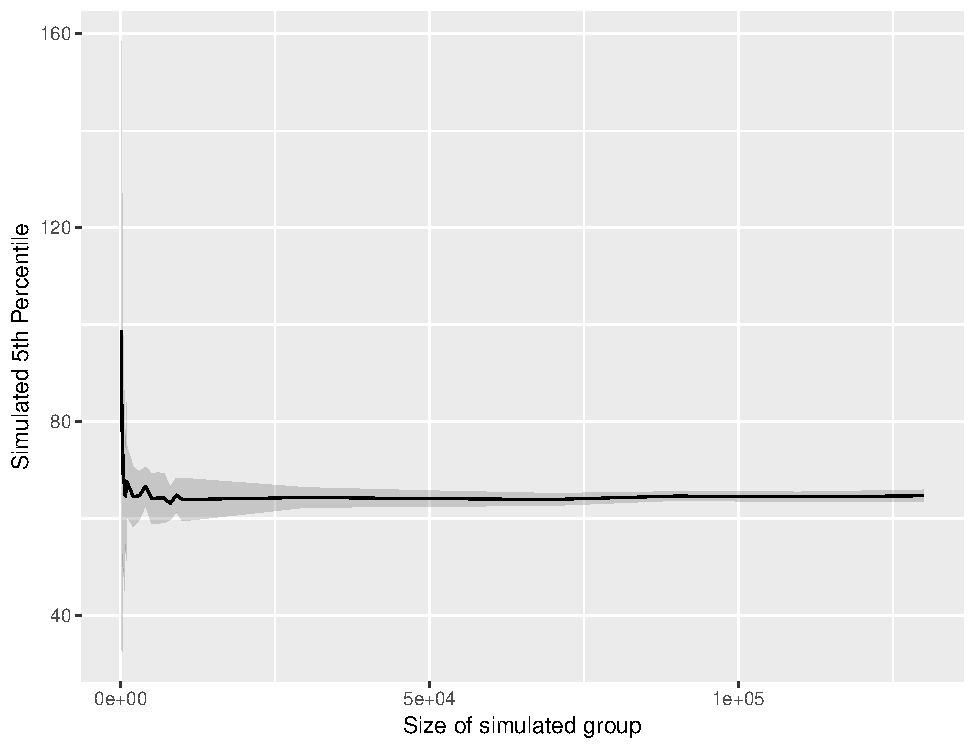
\includegraphics{thesis_files/figure-latex/unnamed-chunk-5-1.pdf}
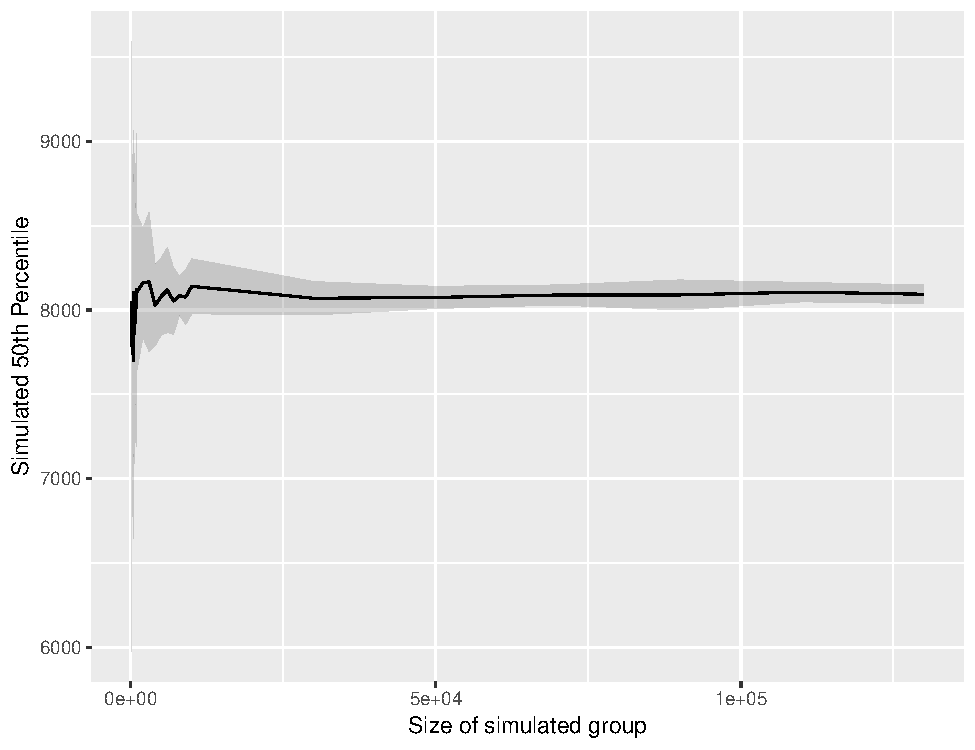
\includegraphics{thesis_files/figure-latex/unnamed-chunk-5-2.pdf}
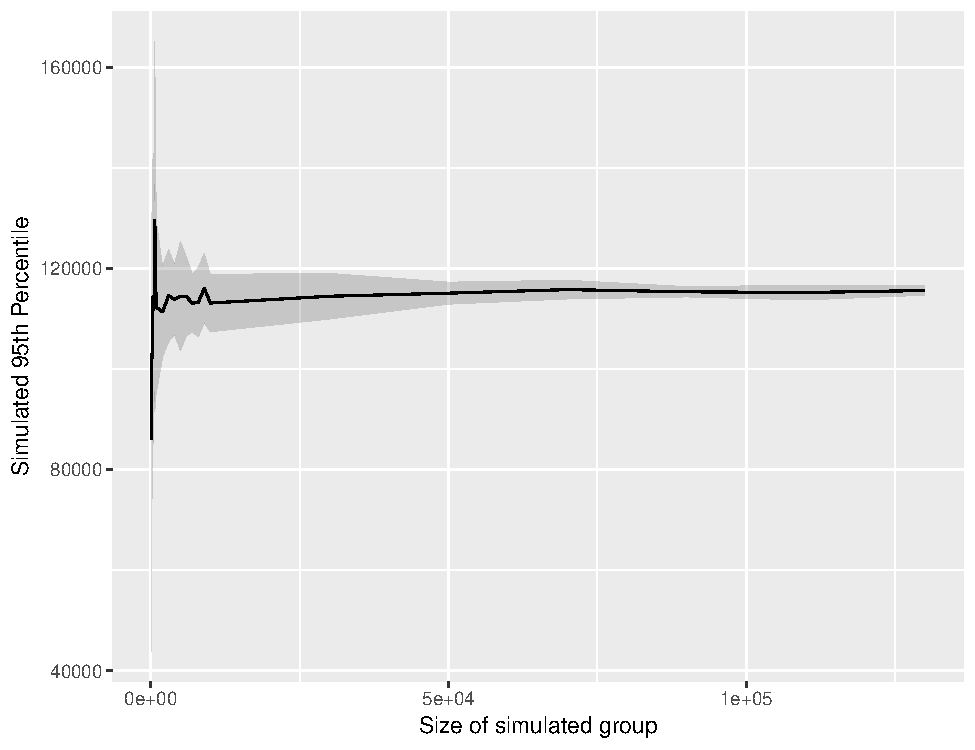
\includegraphics{thesis_files/figure-latex/unnamed-chunk-5-3.pdf}
\begin{Shaded}
\begin{Highlighting}[]
\CommentTok{# ggplot(race_data) + geom_line(aes(x = year, y =}
\CommentTok{# lconcentration, color = (black/pop), group = id), alpha =}
\CommentTok{# 0.3) + labs(x = 'Year', colour = '% Black', title =}
\CommentTok{# 'Toxicity Trend for all Census Tracts')}

\NormalTok{x =}\StringTok{ }\NormalTok{race_data[race_data$year ==}\StringTok{ }\DecValTok{1993} \NormalTok{&}\StringTok{ }\NormalTok{race_data$concentration <}\StringTok{ }
\StringTok{    }\DecValTok{400}\NormalTok{, }\DecValTok{1}\NormalTok{:}\DecValTok{8}\NormalTok{]}
\NormalTok{y =}\StringTok{ }\NormalTok{race_data[race_data$year ==}\StringTok{ }\DecValTok{1994} \NormalTok{&}\StringTok{ }\NormalTok{race_data$concentration <}\StringTok{ }
\StringTok{    }\DecValTok{400}\NormalTok{, }\DecValTok{1}\NormalTok{:}\DecValTok{8}\NormalTok{]}

\KeywordTok{names}\NormalTok{(x) =}\StringTok{ }\KeywordTok{c}\NormalTok{(}\StringTok{"id"}\NormalTok{, }\StringTok{"pop93"}\NormalTok{, }\StringTok{"white93"}\NormalTok{, }\StringTok{"black93"}\NormalTok{, }\StringTok{"native93"}\NormalTok{, }
    \StringTok{"asian93"}\NormalTok{, }\StringTok{"other93"}\NormalTok{, }\StringTok{"concentration93"}\NormalTok{)}
\KeywordTok{names}\NormalTok{(y) =}\StringTok{ }\KeywordTok{c}\NormalTok{(}\StringTok{"id"}\NormalTok{, }\StringTok{"pop94"}\NormalTok{, }\StringTok{"white94"}\NormalTok{, }\StringTok{"black94"}\NormalTok{, }\StringTok{"native94"}\NormalTok{, }
    \StringTok{"asian94"}\NormalTok{, }\StringTok{"other94"}\NormalTok{, }\StringTok{"concentration94"}\NormalTok{)}

\NormalTok{x =}\StringTok{ }\KeywordTok{merge}\NormalTok{(x, y, }\DataTypeTok{by =} \StringTok{"id"}\NormalTok{)}

\NormalTok{z =}\StringTok{ }\NormalTok{(x$concentration94 *}\StringTok{ }\NormalTok{(x$black94/}\KeywordTok{sum}\NormalTok{(x$black94))) -}\StringTok{ }\NormalTok{(x$concentration93 *}\StringTok{ }
\StringTok{    }\NormalTok{(x$black93/}\KeywordTok{sum}\NormalTok{(x$black93)))}

\KeywordTok{ggplot}\NormalTok{(x) +}\StringTok{ }\KeywordTok{geom_point}\NormalTok{(}\KeywordTok{aes}\NormalTok{(}\DataTypeTok{x =} \NormalTok{concentration93, }\DataTypeTok{y =} \NormalTok{concentration94))}
\end{Highlighting}
\end{Shaded}
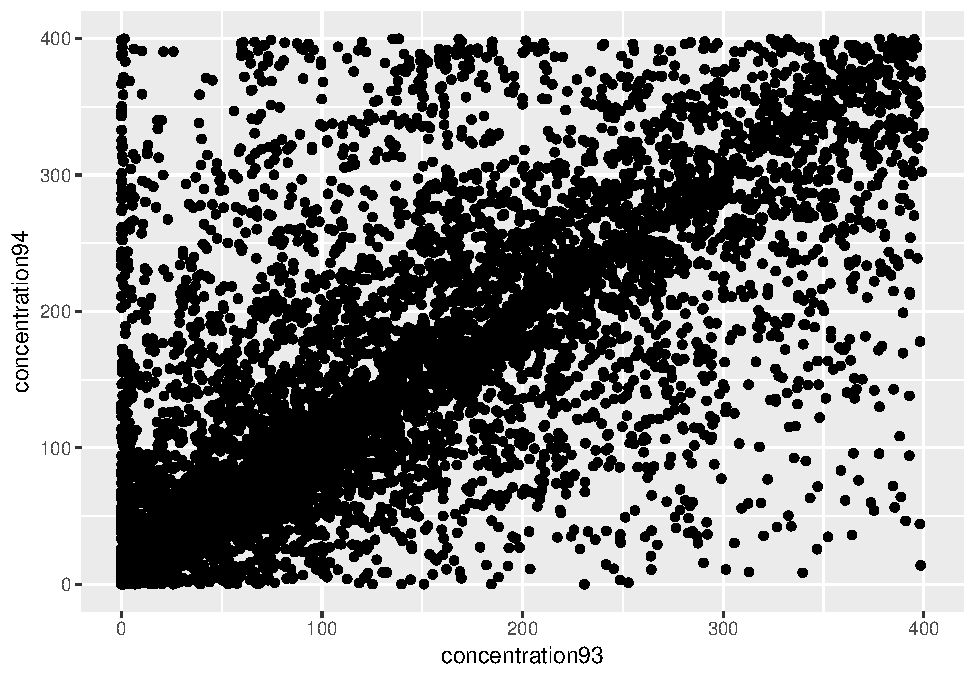
\includegraphics{thesis_files/figure-latex/unnamed-chunk-6-1.pdf}

\chapter{Results}\label{organization}

\chapter*{Conclusion}\label{conclusion}
\addcontentsline{toc}{chapter}{Conclusion}

testing testing

123 hello

\appendix

\chapter{The First Appendix}\label{the-first-appendix}

This first appendix includes all of the R chunks of code that were
hidden throughout the document (using the \texttt{include\ =\ FALSE}
chunk tag) to help with readibility and/or setup.

\textbf{In the main Rmd file}
\begin{Shaded}
\begin{Highlighting}[]
\CommentTok{# This chunk ensures that the thesisdowndss package is}
\CommentTok{# installed and loaded. This thesisdowndss package includes}
\CommentTok{# the template files for the thesis.}
\NormalTok{if (!}\KeywordTok{require}\NormalTok{(devtools)) }\KeywordTok{install.packages}\NormalTok{(}\StringTok{"devtools"}\NormalTok{, }\DataTypeTok{repos =} \StringTok{"http://cran.rstudio.com"}\NormalTok{)}
\NormalTok{if (!}\KeywordTok{require}\NormalTok{(thesisdowndss)) devtools::}\KeywordTok{install_github}\NormalTok{(}\StringTok{"mine-cetinkaya-rundel/thesisdowndss"}\NormalTok{)}
\KeywordTok{library}\NormalTok{(thesisdowndss)}
\KeywordTok{library}\NormalTok{(knitr)}
\NormalTok{opts_chunk$}\KeywordTok{set}\NormalTok{(}\DataTypeTok{tidy.opts =} \KeywordTok{list}\NormalTok{(}\DataTypeTok{width.cutoff =} \DecValTok{60}\NormalTok{), }\DataTypeTok{tidy =} \OtherTok{TRUE}\NormalTok{)}
\KeywordTok{library}\NormalTok{(magrittr)}
\KeywordTok{library}\NormalTok{(readr)}
\KeywordTok{library}\NormalTok{(ggplot2)}
\KeywordTok{library}\NormalTok{(dplyr)}
\KeywordTok{library}\NormalTok{(plyr)}
\KeywordTok{library}\NormalTok{(stringr)}
\KeywordTok{library}\NormalTok{(spatstat)}
\KeywordTok{library}\NormalTok{(readr)}
\KeywordTok{library}\NormalTok{(tidyr)}
\KeywordTok{library}\NormalTok{(devtools)}
\NormalTok{devtools::}\KeywordTok{install_github}\NormalTok{(}\StringTok{"amd112/rseiAnalysis"}\NormalTok{)}
\end{Highlighting}
\end{Shaded}
\begin{verbatim}
Skipping install of 'rseiAnalysis' from a github remote, the SHA1 (19dfcc35) has not changed since last install.
  Use `force = TRUE` to force installation
\end{verbatim}
\begin{Shaded}
\begin{Highlighting}[]
\KeywordTok{library}\NormalTok{(}\StringTok{"rseiAnalysis"}\NormalTok{)}
\CommentTok{# needed for RSEI}
\KeywordTok{set.seed}\NormalTok{(}\DecValTok{4012}\NormalTok{)}
\KeywordTok{library}\NormalTok{(data.table)}
\end{Highlighting}
\end{Shaded}
\textbf{In Chapter \ref{ref-labels}:}

\chapter{The Second Appendix, for
Fun}\label{the-second-appendix-for-fun}

\backmatter

\chapter*{References}\label{references}
\addcontentsline{toc}{chapter}{References}

\markboth{References}{References}

\noindent

\setlength{\parindent}{-0.20in} \setlength{\leftskip}{0.20in}
\setlength{\parskip}{8pt}

\hypertarget{refs}{}
\hypertarget{ref-angel2000}{}
Angel, E. (2000). \emph{Interactive computer graphics : A top-down
approach with opengl}. Boston, MA: Addison Wesley Longman.

\hypertarget{ref-angel2001}{}
Angel, E. (2001a). \emph{Batch-file computer graphics : A bottom-up
approach with quicktime}. Boston, MA: Wesley Addison Longman.

\hypertarget{ref-angel2002a}{}
Angel, E. (2001b). \emph{Test second book by angel}. Boston, MA: Wesley
Addison Longman.


% Index?

\end{document}
